% Options for packages loaded elsewhere
\PassOptionsToPackage{unicode}{hyperref}
\PassOptionsToPackage{hyphens}{url}
%
\documentclass[
]{article}
\usepackage{amsmath,amssymb}
\usepackage{lmodern}
\usepackage{iftex}
\usepackage{graphicx}
\usepackage{float}
\ifPDFTeX
  \usepackage[T1]{fontenc}
  \usepackage[utf8]{inputenc}
  \usepackage{textcomp} % provide euro and other symbols
\else % if luatex or xetex
  \usepackage{unicode-math}
  \defaultfontfeatures{Scale=MatchLowercase}
  \defaultfontfeatures[\rmfamily]{Ligatures=TeX,Scale=1}
\fi
% Use upquote if available, for straight quotes in verbatim environments
\IfFileExists{upquote.sty}{\usepackage{upquote}}{}
\IfFileExists{microtype.sty}{% use microtype if available
  \usepackage[]{microtype}
  \UseMicrotypeSet[protrusion]{basicmath} % disable protrusion for tt fonts
}{}
\makeatletter
\@ifundefined{KOMAClassName}{% if non-KOMA class
  \IfFileExists{parskip.sty}{%
    \usepackage{parskip}
  }{% else
    \setlength{\parindent}{0pt}
    \setlength{\parskip}{6pt plus 2pt minus 1pt}}
}{% if KOMA class
  \KOMAoptions{parskip=half}}
\makeatother
\usepackage{xcolor}
\IfFileExists{xurl.sty}{\usepackage{xurl}}{} % add URL line breaks if available
\IfFileExists{bookmark.sty}{\usepackage{bookmark}}{\usepackage{hyperref}}
\hypersetup{
  pdftitle={arc42 Template},
  hidelinks,
  pdfcreator={LaTeX via pandoc}}
\urlstyle{same} % disable monospaced font for URLs
\usepackage{longtable,booktabs,array}
\usepackage{calc} % for calculating minipage widths
% Correct order of tables after \paragraph or \subparagraph
\usepackage{etoolbox}
\makeatletter
\patchcmd\longtable{\par}{\if@noskipsec\mbox{}\fi\par}{}{}
\makeatother
% Allow footnotes in longtable head/foot
\IfFileExists{footnotehyper.sty}{\usepackage{footnotehyper}}{\usepackage{footnote}}
\makesavenoteenv{longtable}
\usepackage{graphicx}
\makeatletter
\def\maxwidth{\ifdim\Gin@nat@width>\linewidth\linewidth\else\Gin@nat@width\fi}
\def\maxheight{\ifdim\Gin@nat@height>\textheight\textheight\else\Gin@nat@height\fi}
\makeatother
% Scale images if necessary, so that they will not overflow the page
% margins by default, and it is still possible to overwrite the defaults
% using explicit options in \includegraphics[width, height, ...]{}
\setkeys{Gin}{width=\maxwidth,height=\maxheight,keepaspectratio}
% Set default figure placement to htbp
\makeatletter
\def\fps@figure{htbp}
\makeatother
\setlength{\emergencystretch}{3em} % prevent overfull lines
\providecommand{\tightlist}{%
  \setlength{\itemsep}{0pt}\setlength{\parskip}{0pt}}
\setcounter{secnumdepth}{-\maxdimen} % remove section numbering
\ifLuaTeX
  \usepackage{selnolig}  % disable illegal ligatures
\fi

\usepackage[citestyle=numeric, sorting=none]{biblatex}


\addbibresource{Literatur.bib}

\title{
\includegraphics{resources/header.png} Projektbericht Trashpong}
\author{}
\date{Januar 2023}

\begin{document}
\maketitle

% DOCUMENT STARTS HERE
\hypertarget{section-introduction-and-goals}{%
\section{Architektur}\label{section-introduction-and-goals}}

Im Rahmen der Architektur wird eine zentralisierte Architektur verwendet, wobei es sich um eine Client-Server-Architektur handelt (vgl. Abbildung \ref{fig:clientserver}).
Die Programmteile werden in zwei separate Einheiten unterteilt, um eine klare Trennung zu gewährleisten. Der Server stellt einen bestimmten Service bereit und leitet die Anfragen an die Clients weiter. Die Clients empfangen diese Anfragen.\cite{tanenbaum2007distributed}

Der Client ist eine kompilierte Executable, geschrieben in der Open-Source Godot Engine \cite{godot}. Dort befindet sich die Gesamte Spiel Logik über die der Benutzer das Spiel spielen kann. Der Server befindet sich in einem Docker Compose bestehend aus einer Posgres Datenbank, einem Load Balancer und beliebig skalierbare Spieleserver welche die Anfragen der Clients verarbeiten. 
\begin{figure}[H]
	\centering
	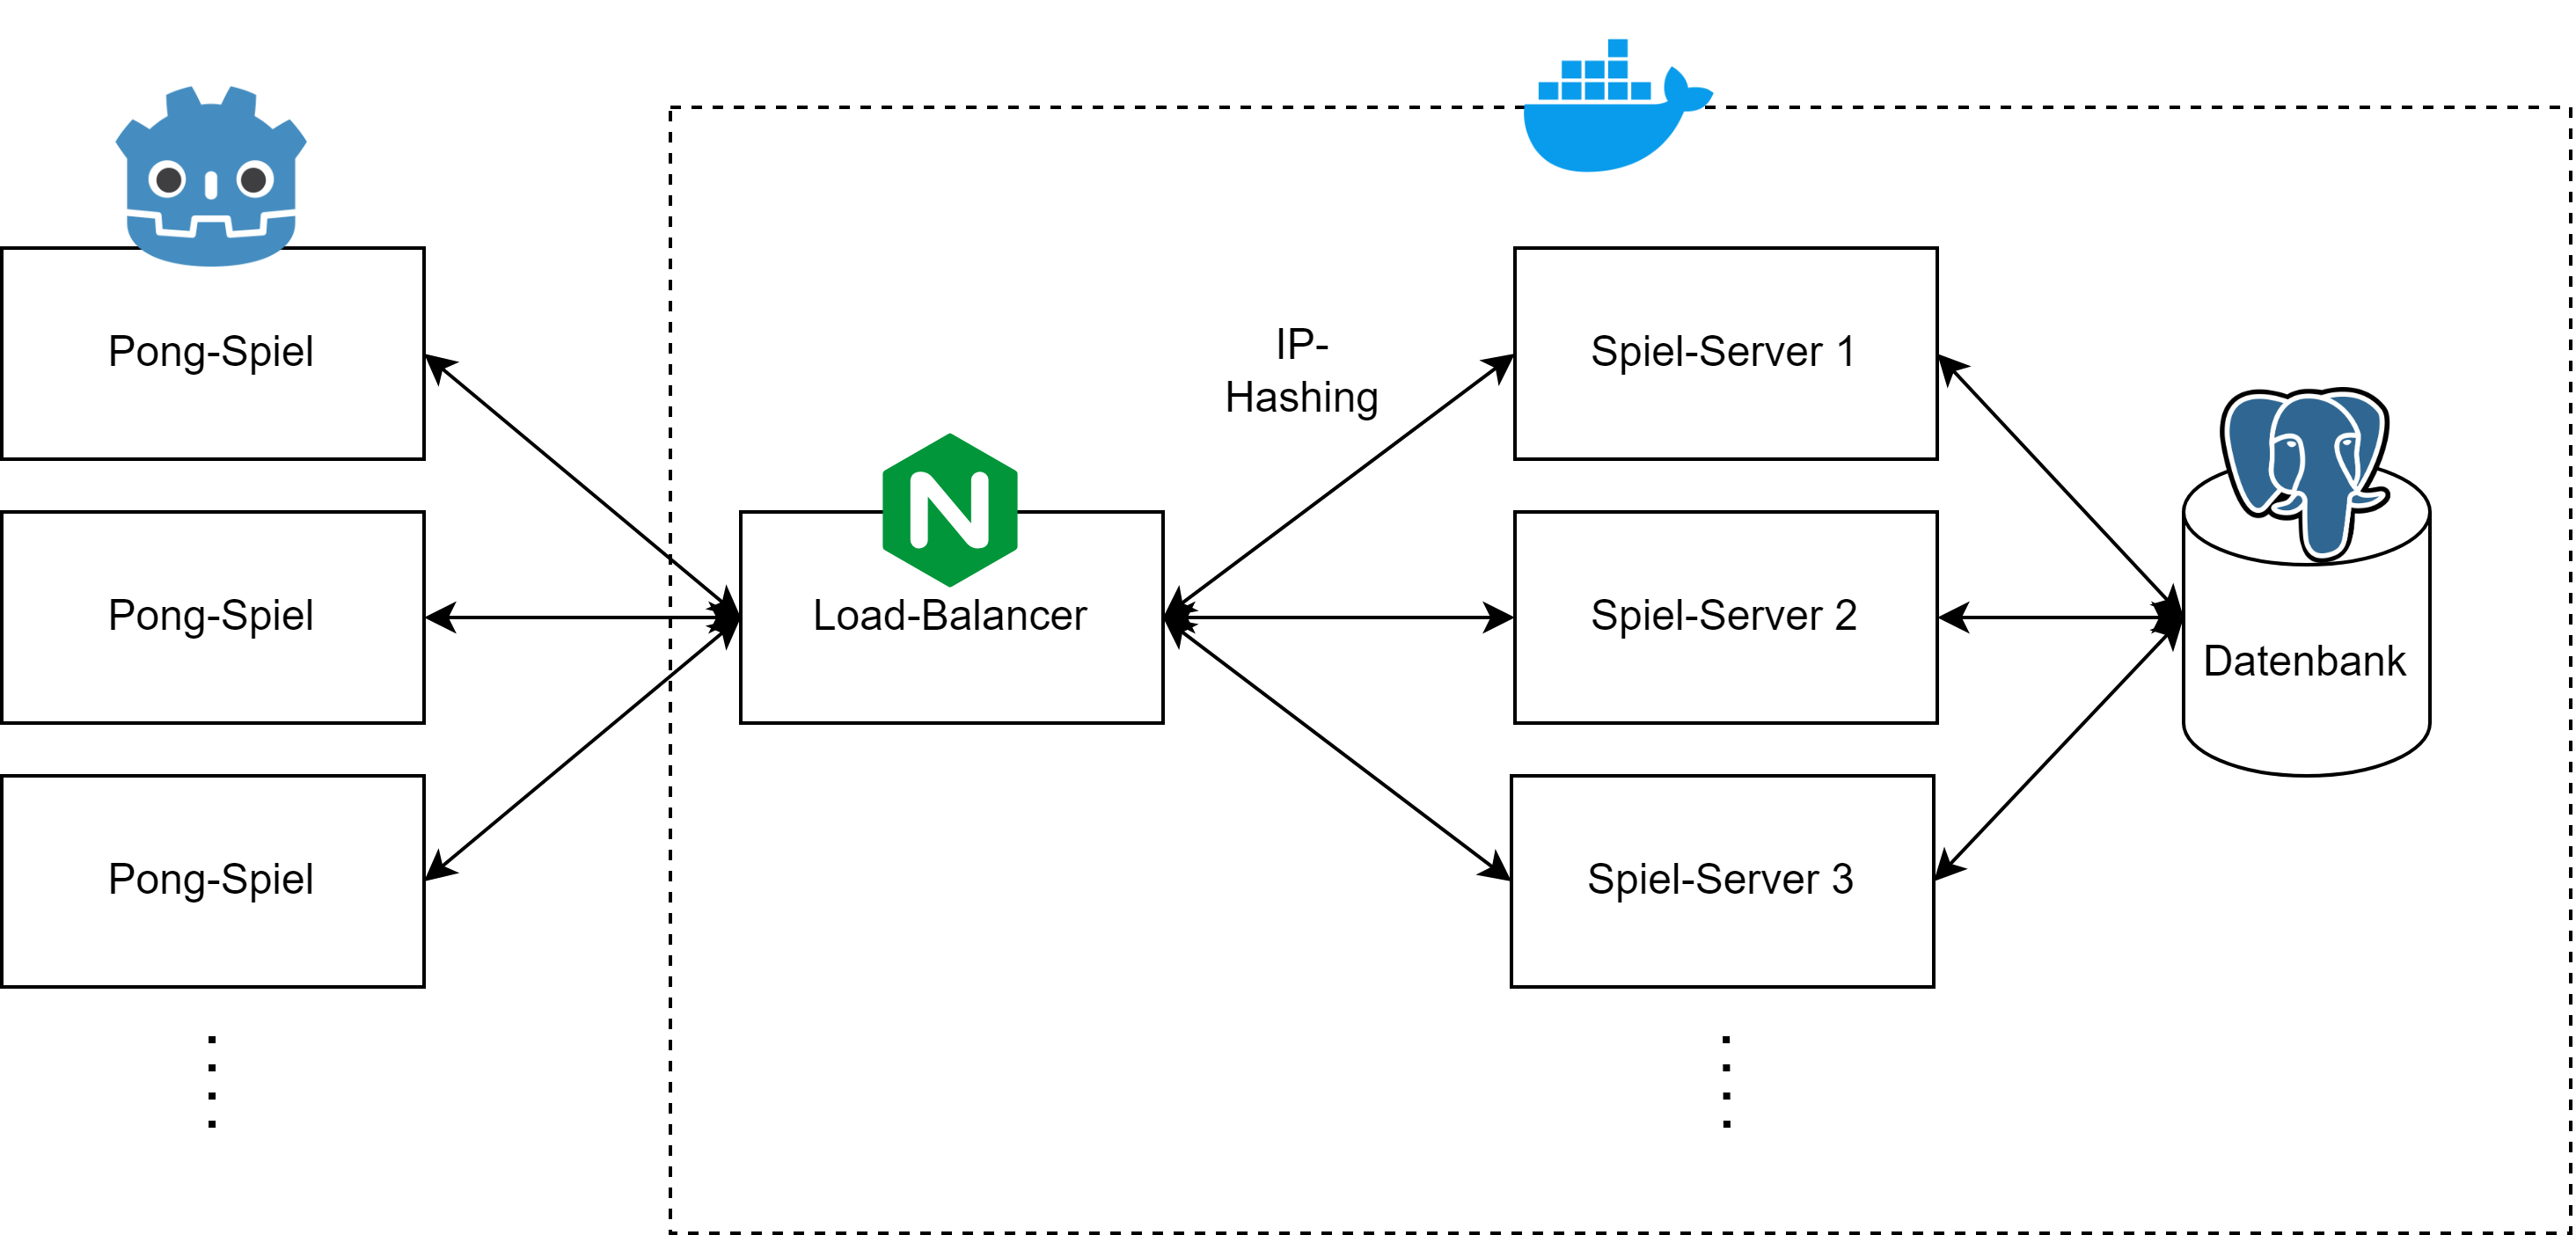
\includegraphics[width=\textwidth ]{resources/Client-Server.drawio.png}
	\caption{Kontext-Sicht der Client-Server-Architektur des Pong Spiels}
	\label{fig:clientserver}
\end{figure}
Die Datenbank speichert die Räume in der die Spieler ihr Spiel spielen. Jeder Spieler kann Räume erstellen und ihnen beitreten und gehört somit diesen Räumen an (vgl. Abbildung \ref{fig:ER-Modell}). Ein Spieler kann zwar mehrere Räume erstellen, zum Zeitpunkt des Spiels befindet sich dieser nur in einem einzigen Raum.
\begin{figure}[H]
	\centering
	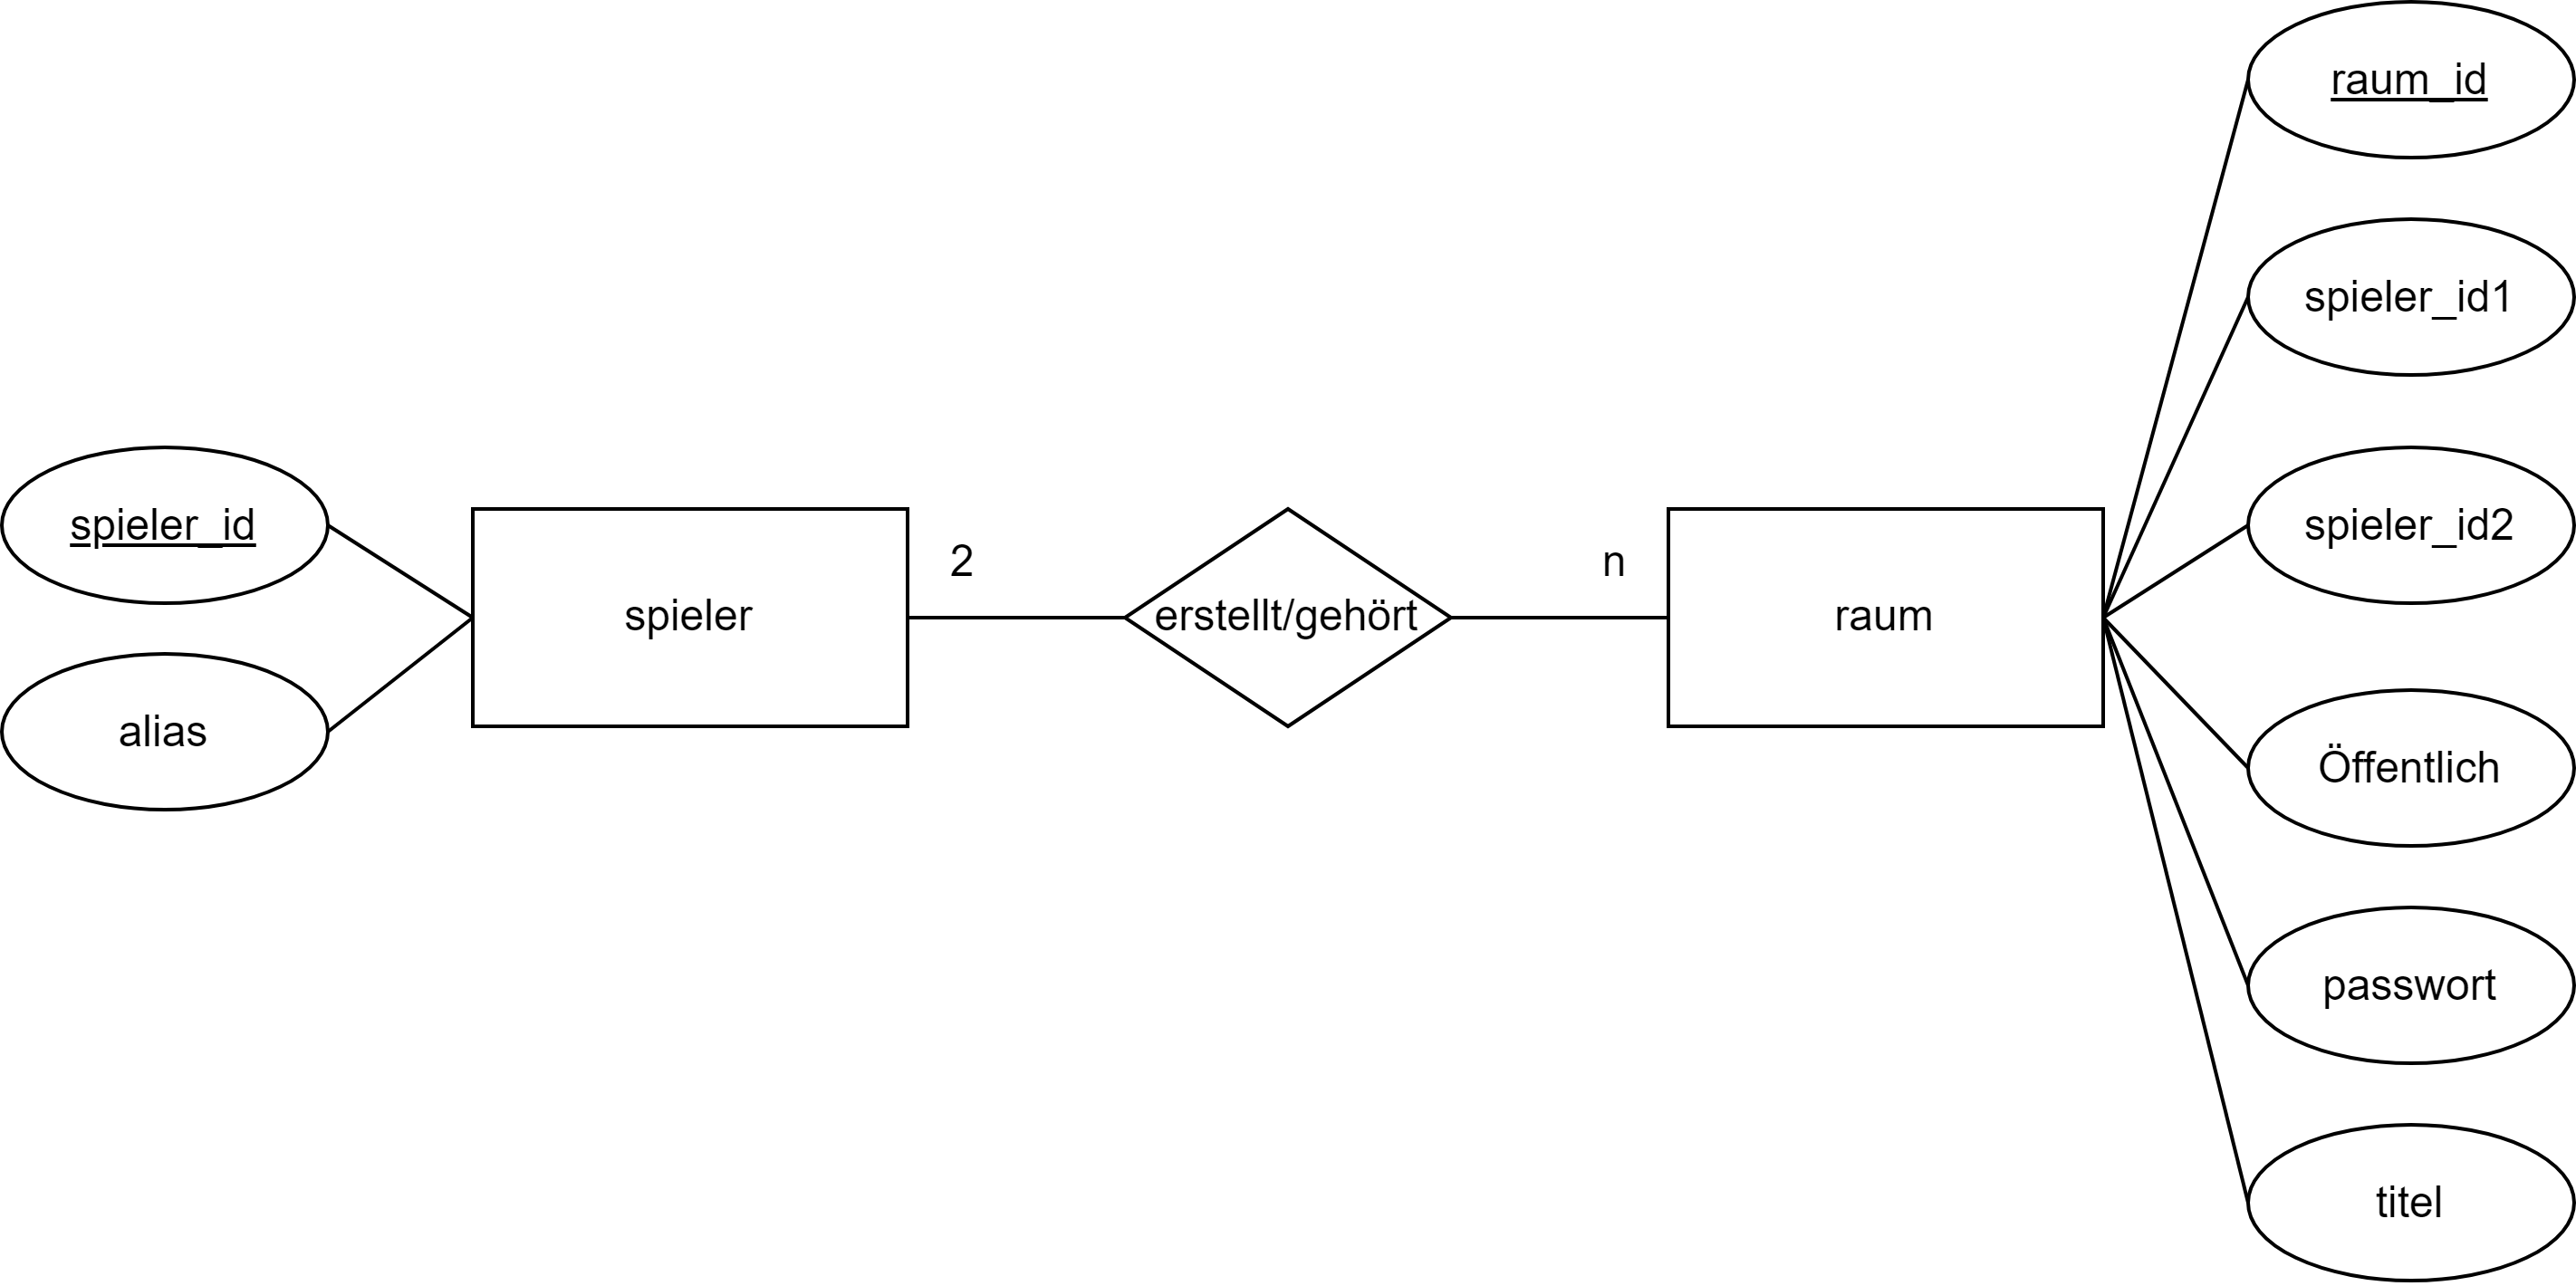
\includegraphics[width=\textwidth ]{resources/ER-Modell.png}
	\caption{ER-Modell der Datenbankarchitektur}
	\label{fig:ER-Modell}
\end{figure}

Dieser verwaltet die Daten der Spieler und die Spielstände. Außerdem werden die Daten für die Räume gespeichert.
Die REST API ist in einem Docker Container gehostet und kann beliebig skaliert werden. 
Ein NGINX Load Balancer verteilt die Anfragen auf die einzelnen Server.
"Viele Client-Server-Anwendung sind grundsetzlich aus drei unterschiedlichen Komponenten zusammengesetzt[...]" \cite[S.57 ff.]{tanenbaum2007distributed}.
So interagieren auch die Clients mit einer Benutzerschnittstelle, der REST API.
Diese wird verwendet um Daten über Nutzer oder Räume zu erhalten.
Daten werden dabei über das HTTP Protokoll ausgetauscht. 
Die REST API kann dabei verwendet werde um Räume zu erstellen.
Die REST Schnittstelle interagiert dabei mit Controllern, die die Logik der Anwendung implementieren und welche dann
mit der Datenhaltung interagieren. Damit kann eine klare Trennung von Datenhaltung und Logik erreicht werden, welches die Anwendung
modular macht. Es können dadurch andere Datenbanksysteme verwendet werden, ohne dass die Logik der Anwendung angepasst werden muss.

Die Abbildung \ref{fig:ablaufdiagramm-show_lobby} zeigt den Ablauf einer REST Anfrage um die Räume zu erhalten.
Hierbei interagiert der Client mit der REST API, welche die Anfrage an den Controller weiterleitet.
Der Controller interagiert dann mit der Datenbank um die Räume zu erhalten. Anschließend werden die Daten an den Client zurückgegeben.

Die Verteilung der Anwendungslogik auf Client und Server wird durch die Abbildung \ref{fig:destribution-of-logic} verdeutlicht.
Diese ist ein ausschnitt aus der Abbildung 2.5(c) aus \cite[S.41]{tanenbaum2007distributed}

Die Benutzerschnittstelle ist hierbei die kompilierte Godot Anwendung, welche die Spiellogik implementiert.
Um Daten zu erhalten, sendet die Anwendung Anfragen an die REST API, welche Anwendungslogik implementiert hat um mit der Datenbank zu interagieren.
Die Benutzeranwendung muss zudem eigene Logik implementieren, da diese aufgrund von Echtzeit Anforderungen nicht auf einen Server warten kann.
Komponenten mit Echtzeit Anforderungen, die das Rendering, die übernahme von Benutzer eingaben müssen auf dem Client Computer ausgeführt werden.


\begin{figure}[H]
	\centering
	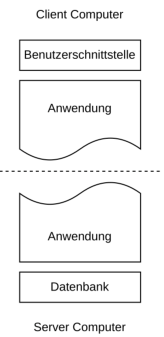
\includegraphics[width=0.8\textwidth ]{resources/server_client.pdf}
	\caption{Aufteilung der Anwendungslogik in Client und Server}
	\label{fig:destribution-of-logic}
\end{figure}


\hypertarget{section-achitactural-decision}{%
\subsection{Architektur Entscheidung}}
Erklärung, warum diese Architektur gewählt wurde (z. B. Skalierbarkeit, Modularität, Sicherheit).

Innerhalb der Server Applikation setzen wir auf zwei Paradigmen. Einerseits haben wir uns bei der Datenhaltung
für ein zentrlisiertes Client Server Modell entschieden. 
Dabei ist der Server "ein Prozess der einen bestimmt Dienst implementiert" \cite[S.55 ff.]{tanenbaum2007distributed}.
In Fall von Trash Pong ist dies eine REST API, die für die Datenhaltung zuständig ist.

Die zentralisierte Form hilft dabei 



\section{Systemkomponenten}

\subsection{Anforderungen}
\begin{center}
  \begin{tabular}{|p{\linewidth}|}
    \hline
    \textbf{Spieler-Registrierung und -Login (FA1)} \\
    Beschreibung: Benutzer müssen sich mit ihren Namen anmelden können, um am Spiel teilzunehmen.
    Die Nutzung sollte niederschwelling sein. Ein Benutzer muss deshalb kein Konto anlegenc \\ \\
    \hline
    \textbf{Echtzeit-Multiplayer-Funktionalität (FA2)} \\
    Beschreibung: Das Spiel muss in der Lage sein, mehrere Spieler in Echtzeit zu verbinden und ein synchronisiertes Spiel zu ermöglichen. Die Bewegungen der Schläger und der Ball müssen in Echtzeit zwischen den Spielern synchronisiert werden.\\ \\
    \hline
    \textbf{Punkteverwaltung (FA3)} \\
    Beschreibung: Das System muss die Punkte der Spieler während des Spiels erfassen und verwalten können. Nach jedem Spiel sollte ein Punktestand angezeigt werden, der den Gewinner ermittelt. \\ \\
    \hline
  \end{tabular}
\end{center}

\begin{center}
  \begin{tabular}{|p{\linewidth}|}
    \hline
    \textbf{Leistung und Skalierbarkeit (NF1)} \\
    Beschreibung: Das Spiel sollte auch bei hoher Benutzerzahl flüssig und ohne Verzögerungen laufen. Das System muss skalierbar sein, um eine große Anzahl von gleichzeitigen Spielern zu unterstützen. \\ \\
    \hline
    \textbf{Sicherheit (NF2)} \\
    Beschreibung: Die Benutzerdaten, einschließlich Anmeldedaten und Spielstatistiken, müssen sicher gespeichert und übertragen werden. Das System sollte gegen häufige Sicherheitsbedrohungen wie SQL-Injektionen und Cross-Site-Scripting geschützt sein.\\ \\
    \hline
    \textbf{Datensparsamkeit (NF3)} \\
     Beschreibung:
     Die Datenerhebung und -speicherung wird nur im notwendigen Maß durchgeführt. 
     Ziel ist es, nur die Daten zu erfassen und zu speichern, die für den Betrieb und die Funktionalität des Systems unbedingt erforderlich sind. 
     Dies trägt zum Schutz der Privatsphäre der Nutzer bei und reduziert das Risiko von Datenmissbrauch und -verlust.
     Deshalb sollen nur der Nutzername und die Punkte gespeichert werden.
    \\ \\
    \hline
    \textbf{Benutzerfreundlichkeit (NF4)} \\
    Beschreibung: Die Benutzeroberfläche des Spiels sollte intuitiv und leicht zu bedienen sein. Neue Spieler sollten sich schnell zurechtfinden und das Spiel ohne umfangreiche Anleitungen verstehen können.\\ \\
    \\ \\
    \hline
  \end{tabular}
\end{center}

\section{Umsetzung}

\subsection{Implementierung}
\begin{itemize}
    \item \textbf{Umsetzung der Architektur}: Beschreibung der Implementierung der einzelnen Komponenten und ihrer Interaktionen.
    \item \textbf{Schwierigkeiten und Lösungen}: Was waren die technischen Herausforderungen und wie wurden sie bewältigt?
\end{itemize}

\begin{figure}[H]
	\centering
	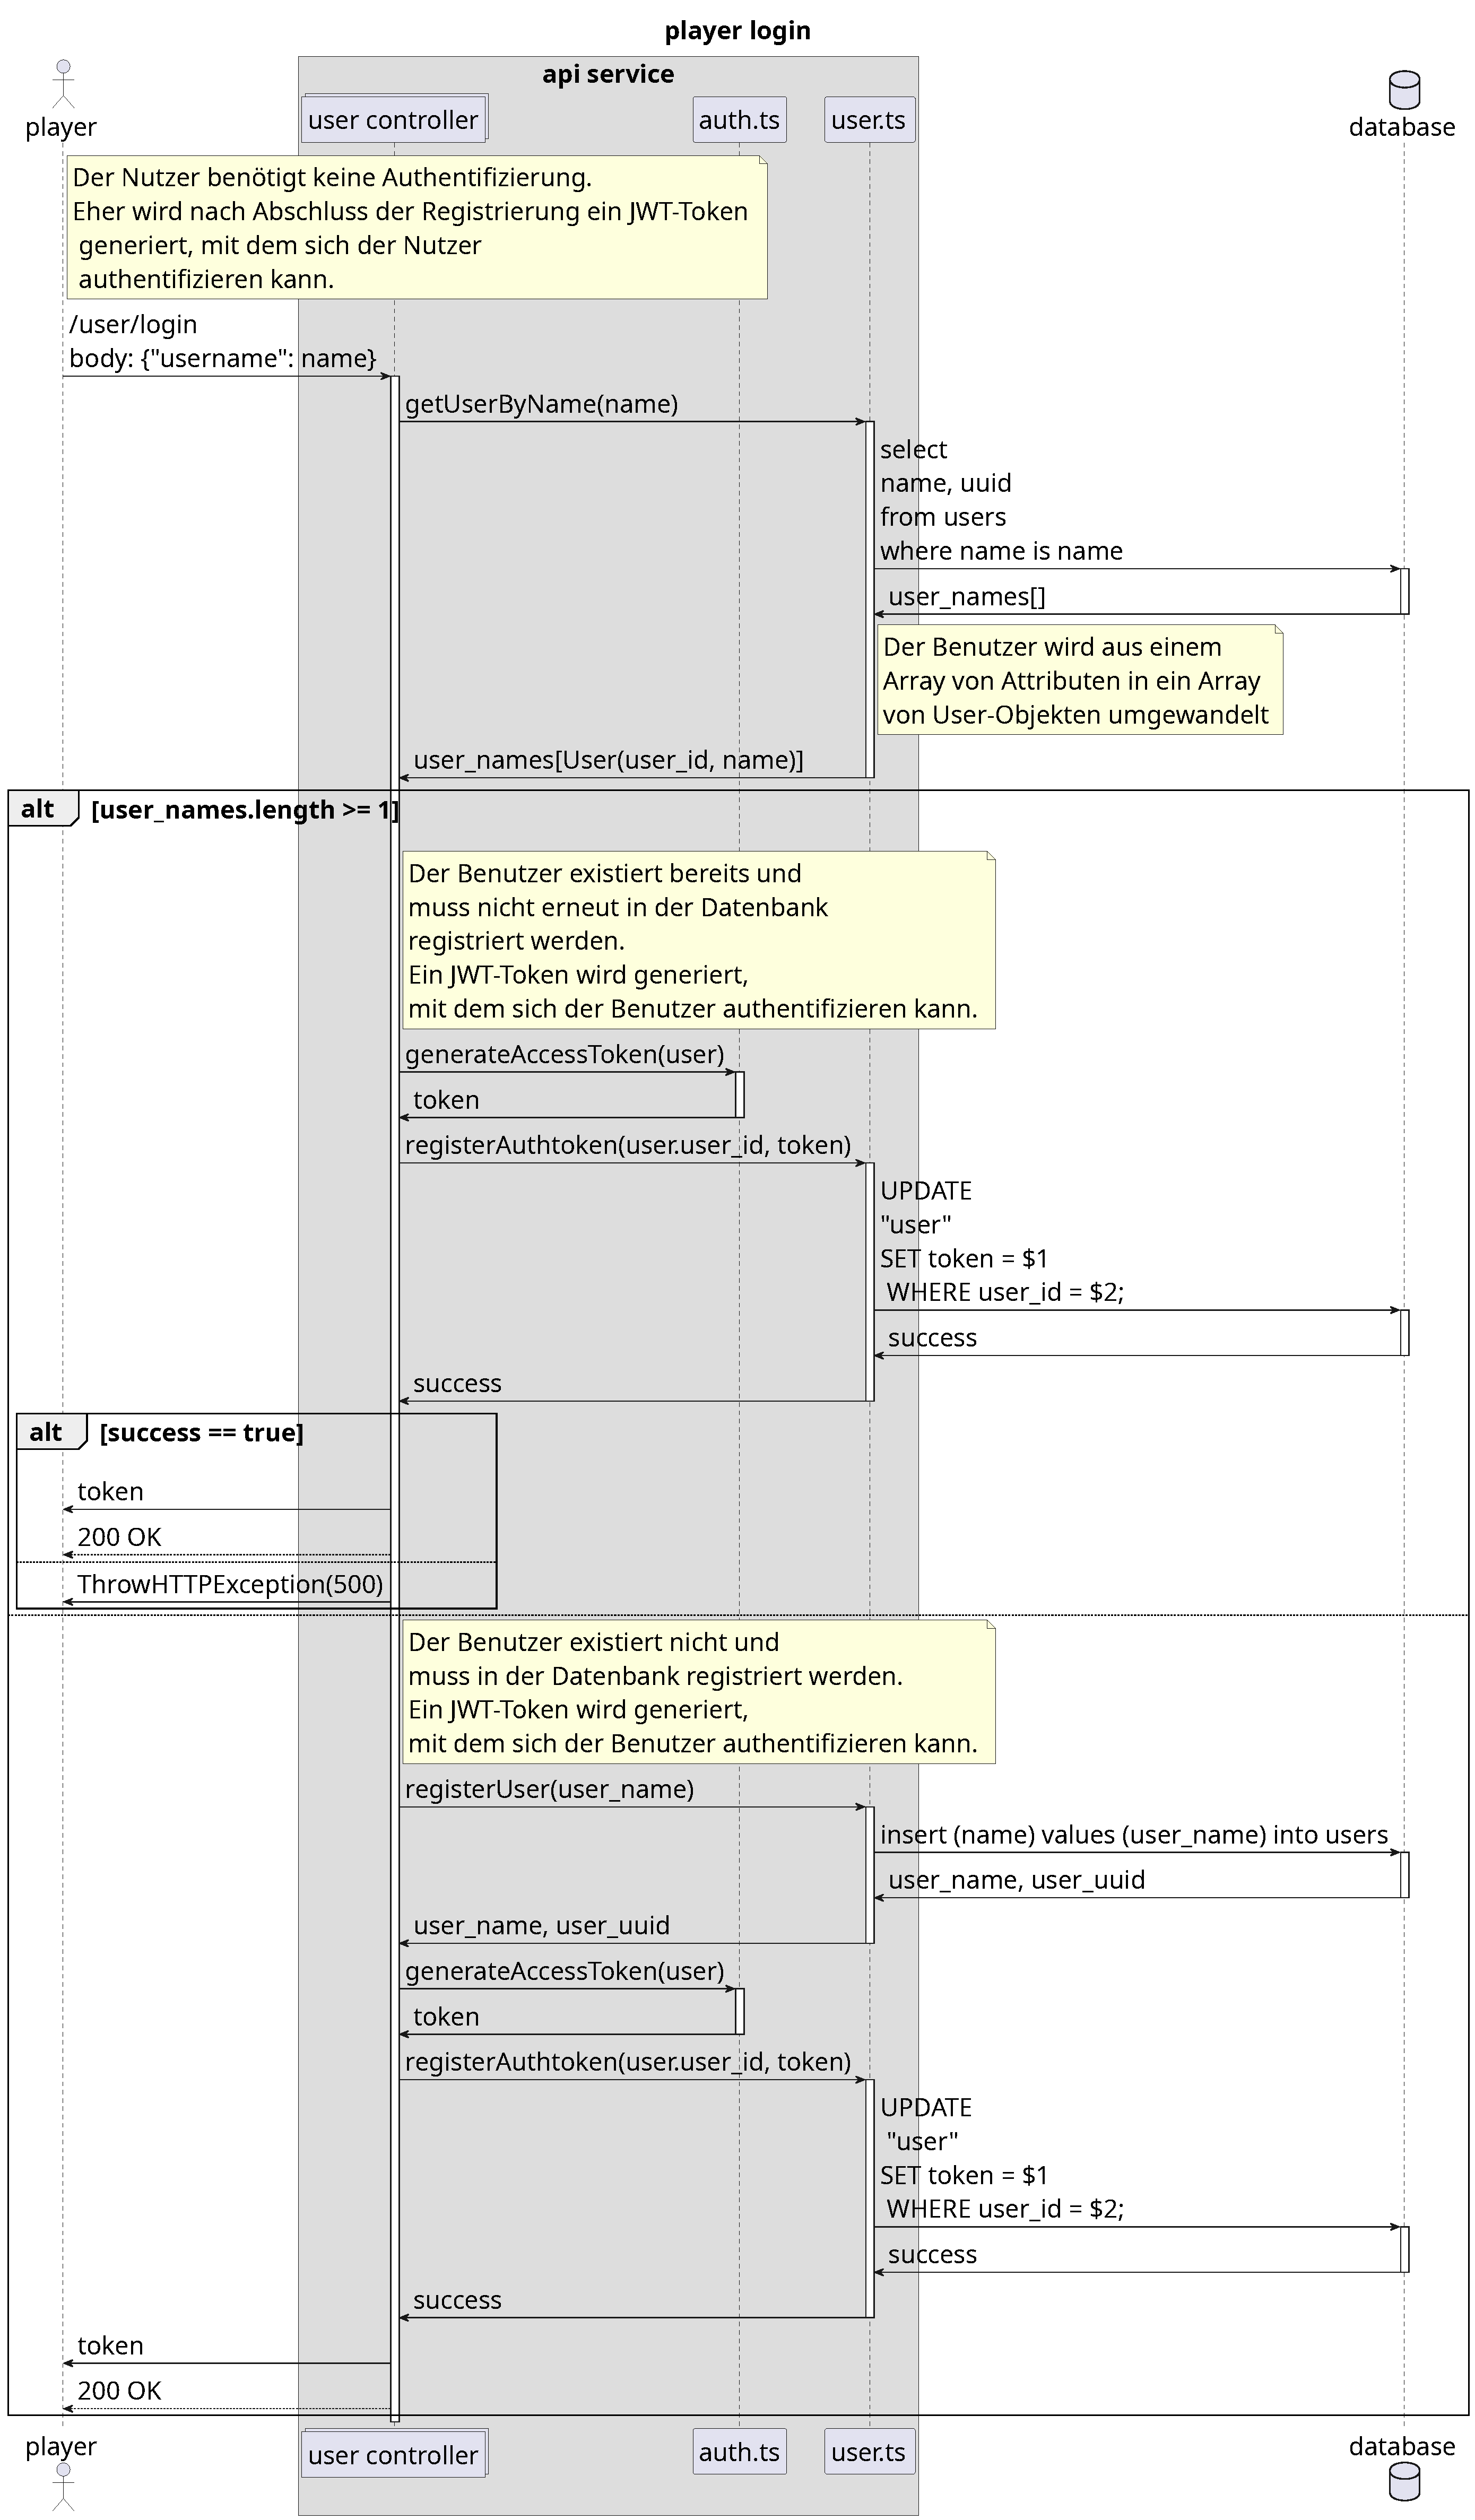
\includegraphics[width=\textwidth ]{resources/login.pdf}
	\caption{Dein TExt hier}
	\label{fig:ablaufdiagramm-login}
\end{figure}
\begin{figure}[H]
	\centering
	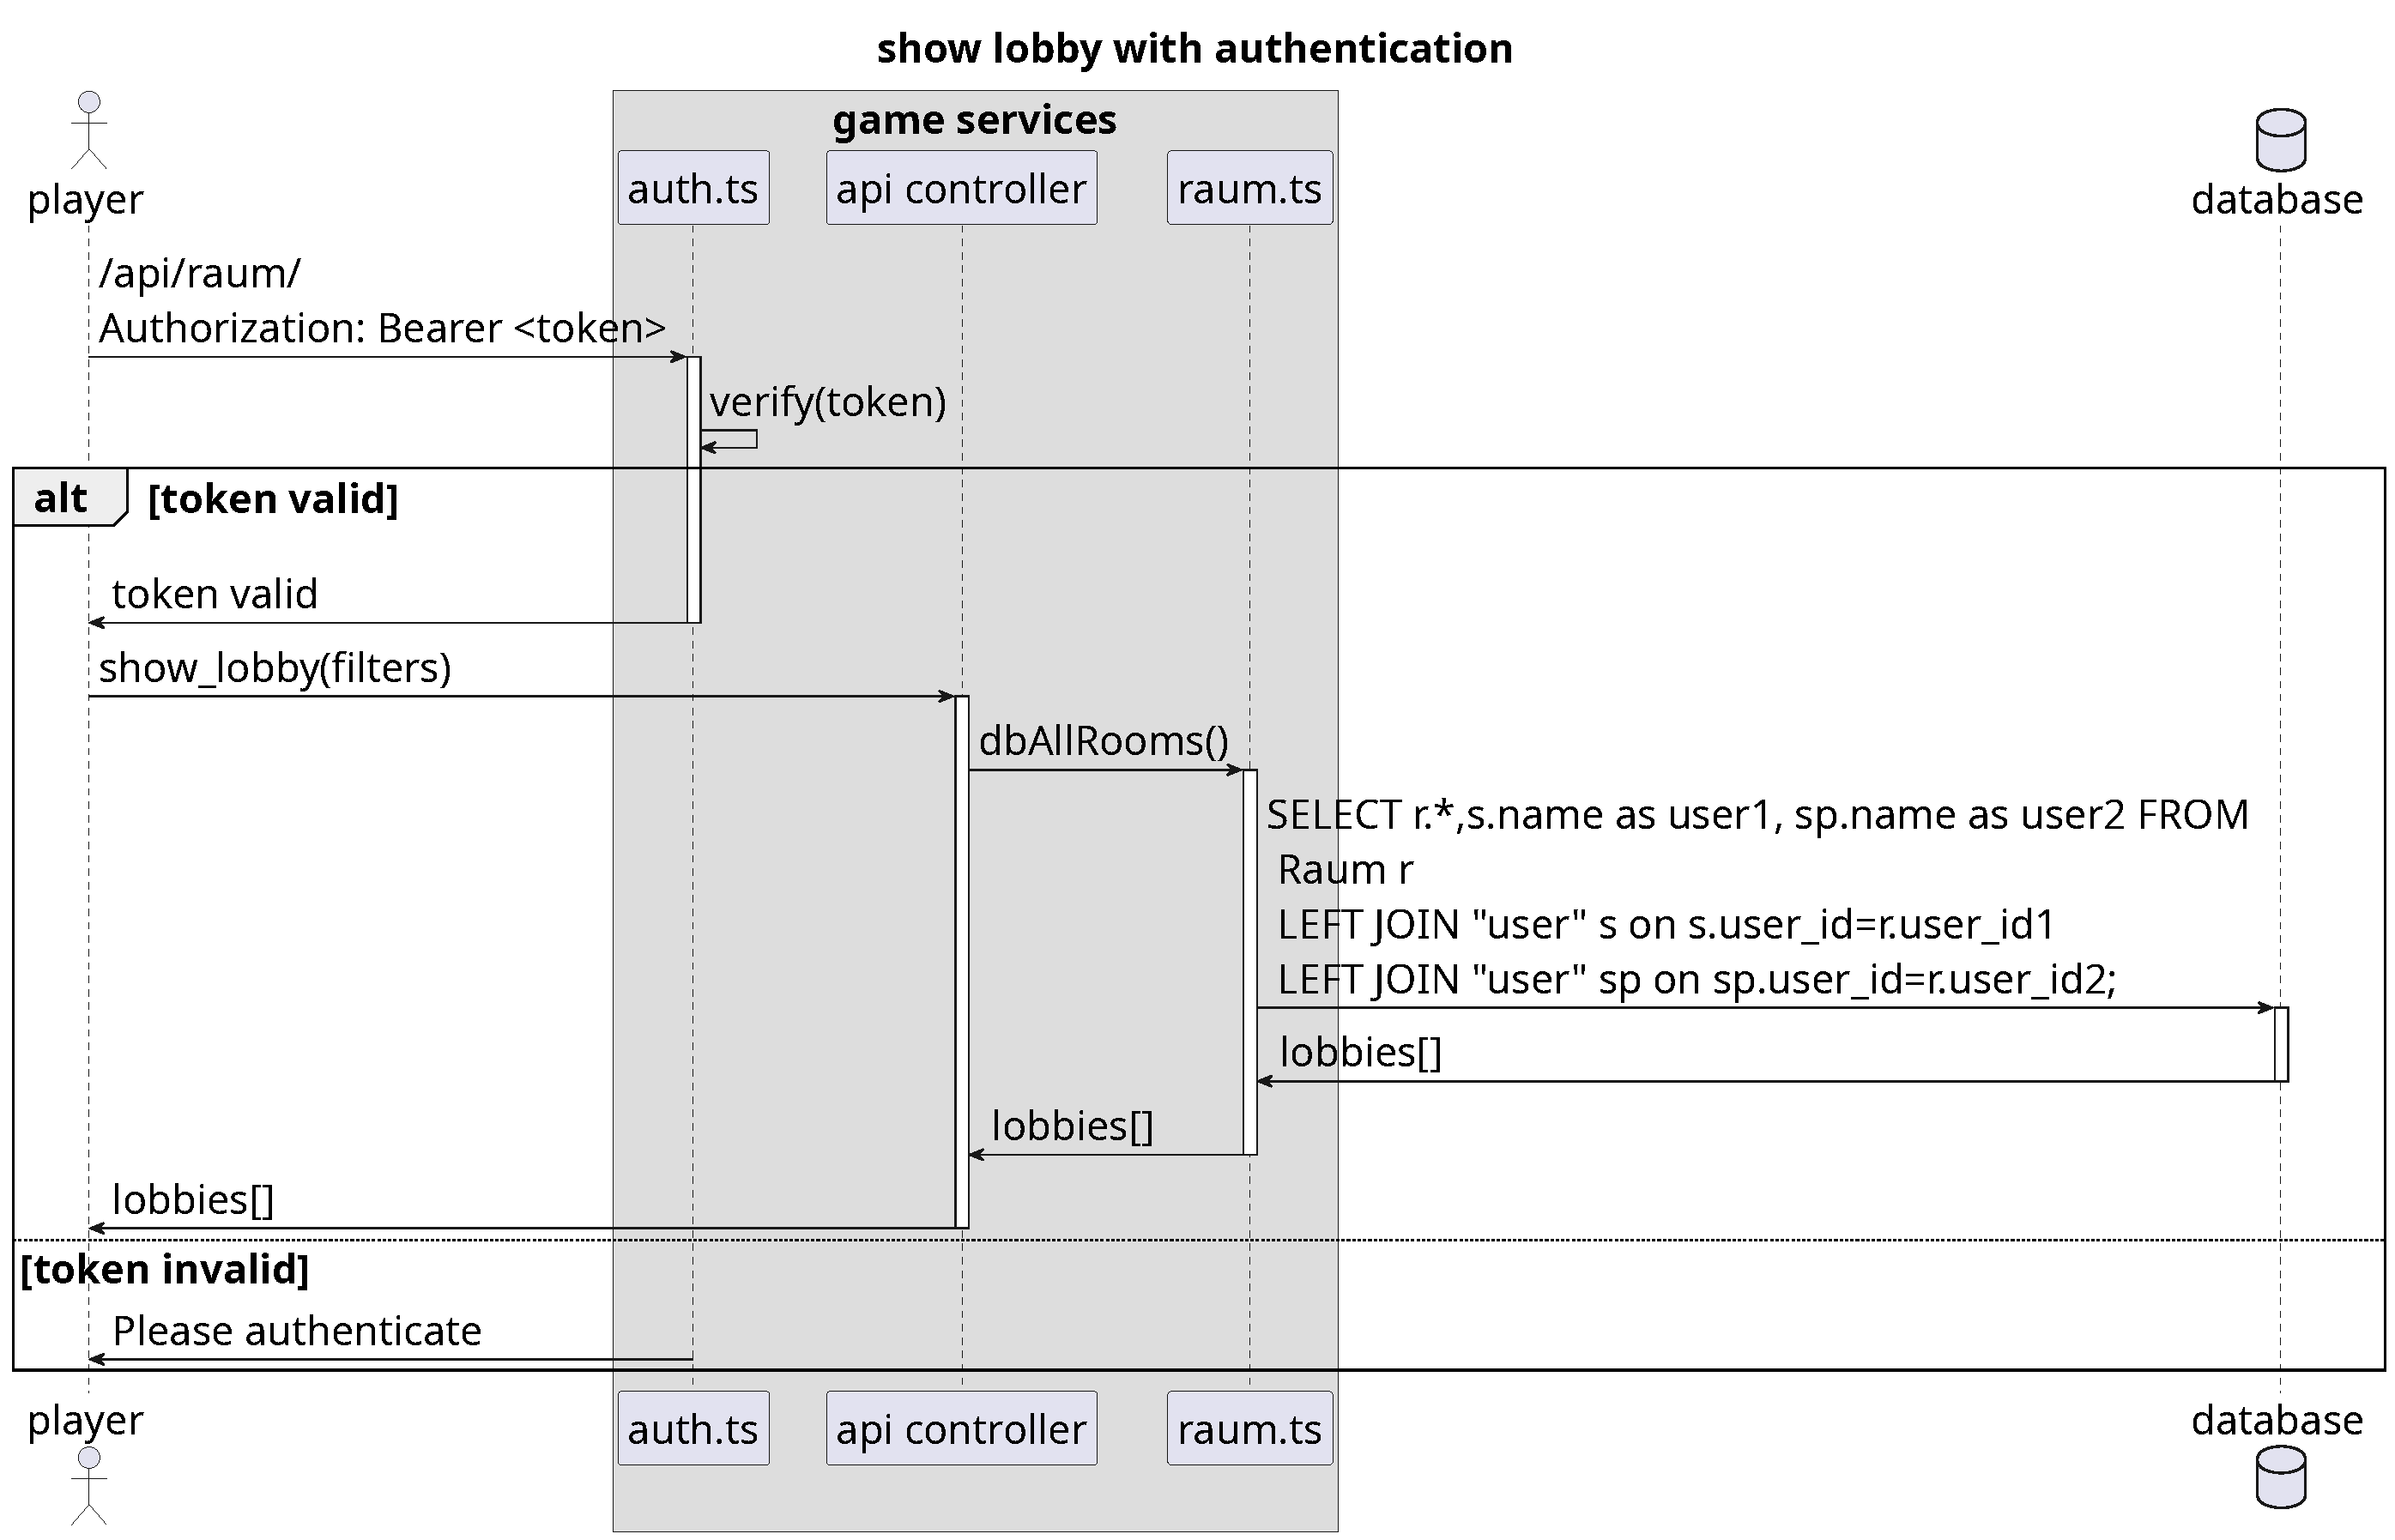
\includegraphics[width=\textwidth ]{resources/show_lobby.pdf}
	\caption{Dein TExt hier}
	\label{fig:ablaufdiagramm-show_lobby}
\end{figure}
\begin{figure}[H]
	\centering
	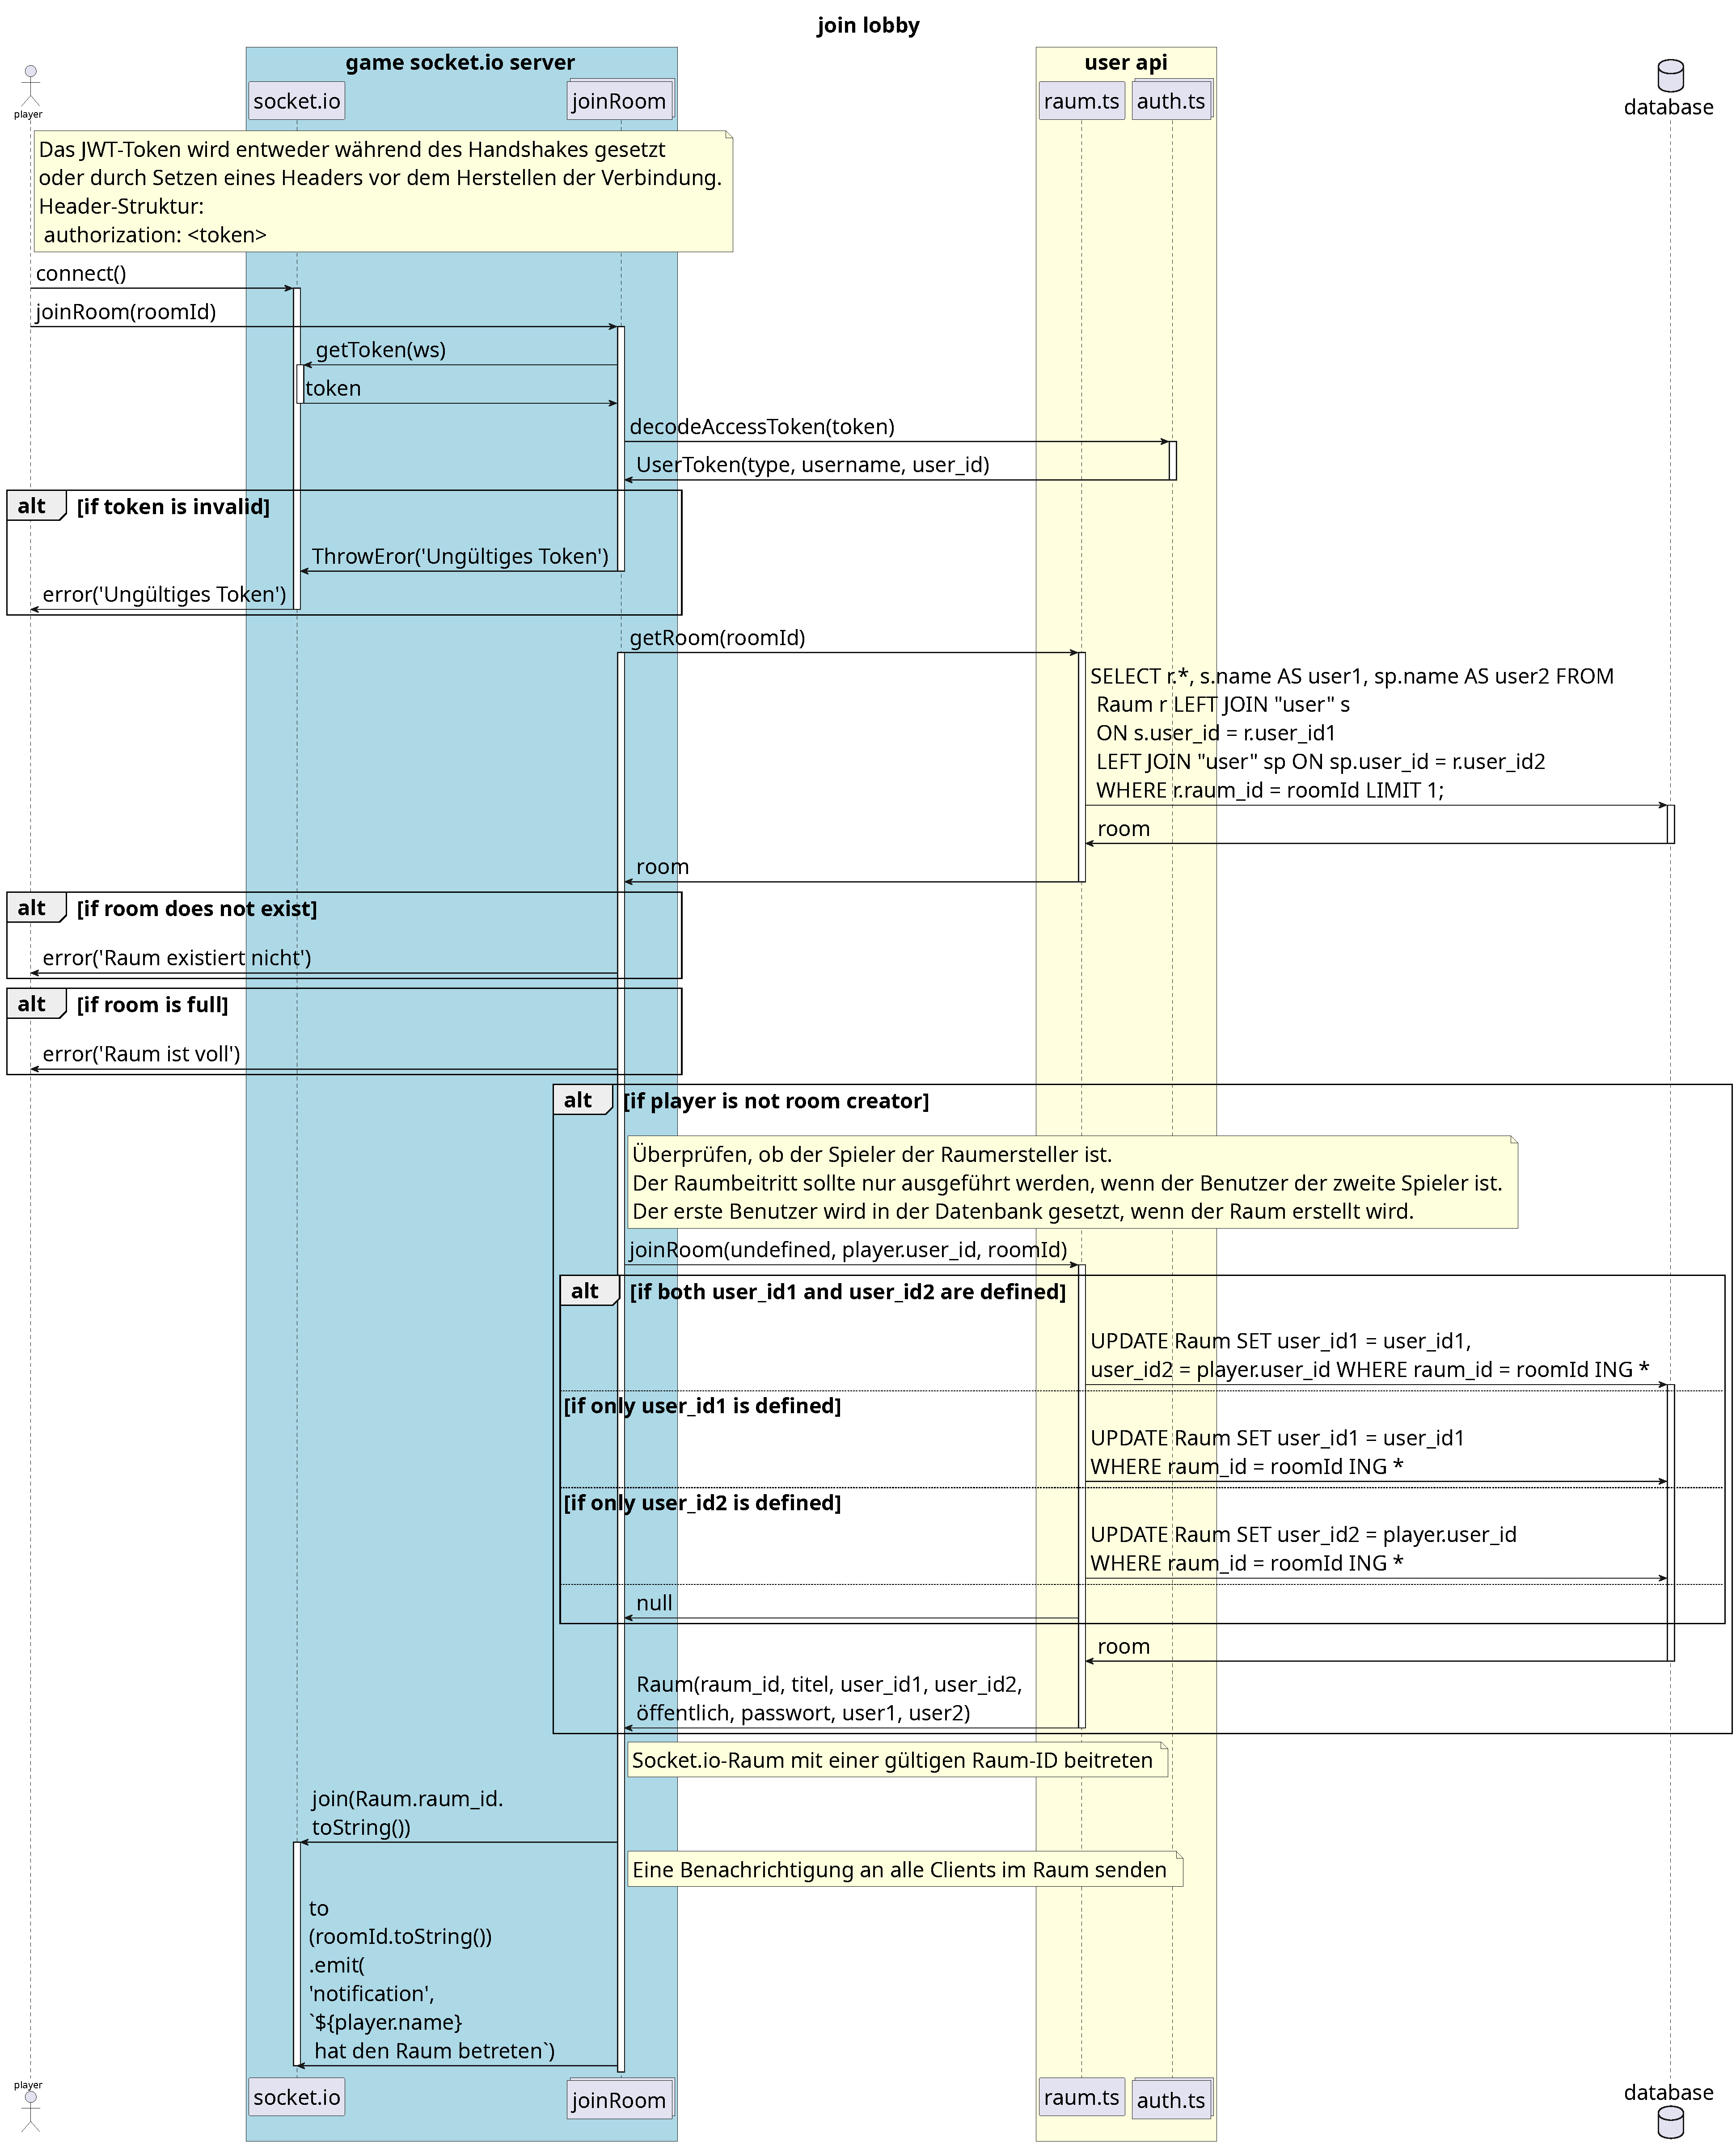
\includegraphics[width=\textwidth ]{resources/join_lobby.pdf}
	\caption{Dein TExt hier}
	\label{fig:ablaufdiagramm-join_lobby}
\end{figure}
\begin{figure}[H]
	\centering
	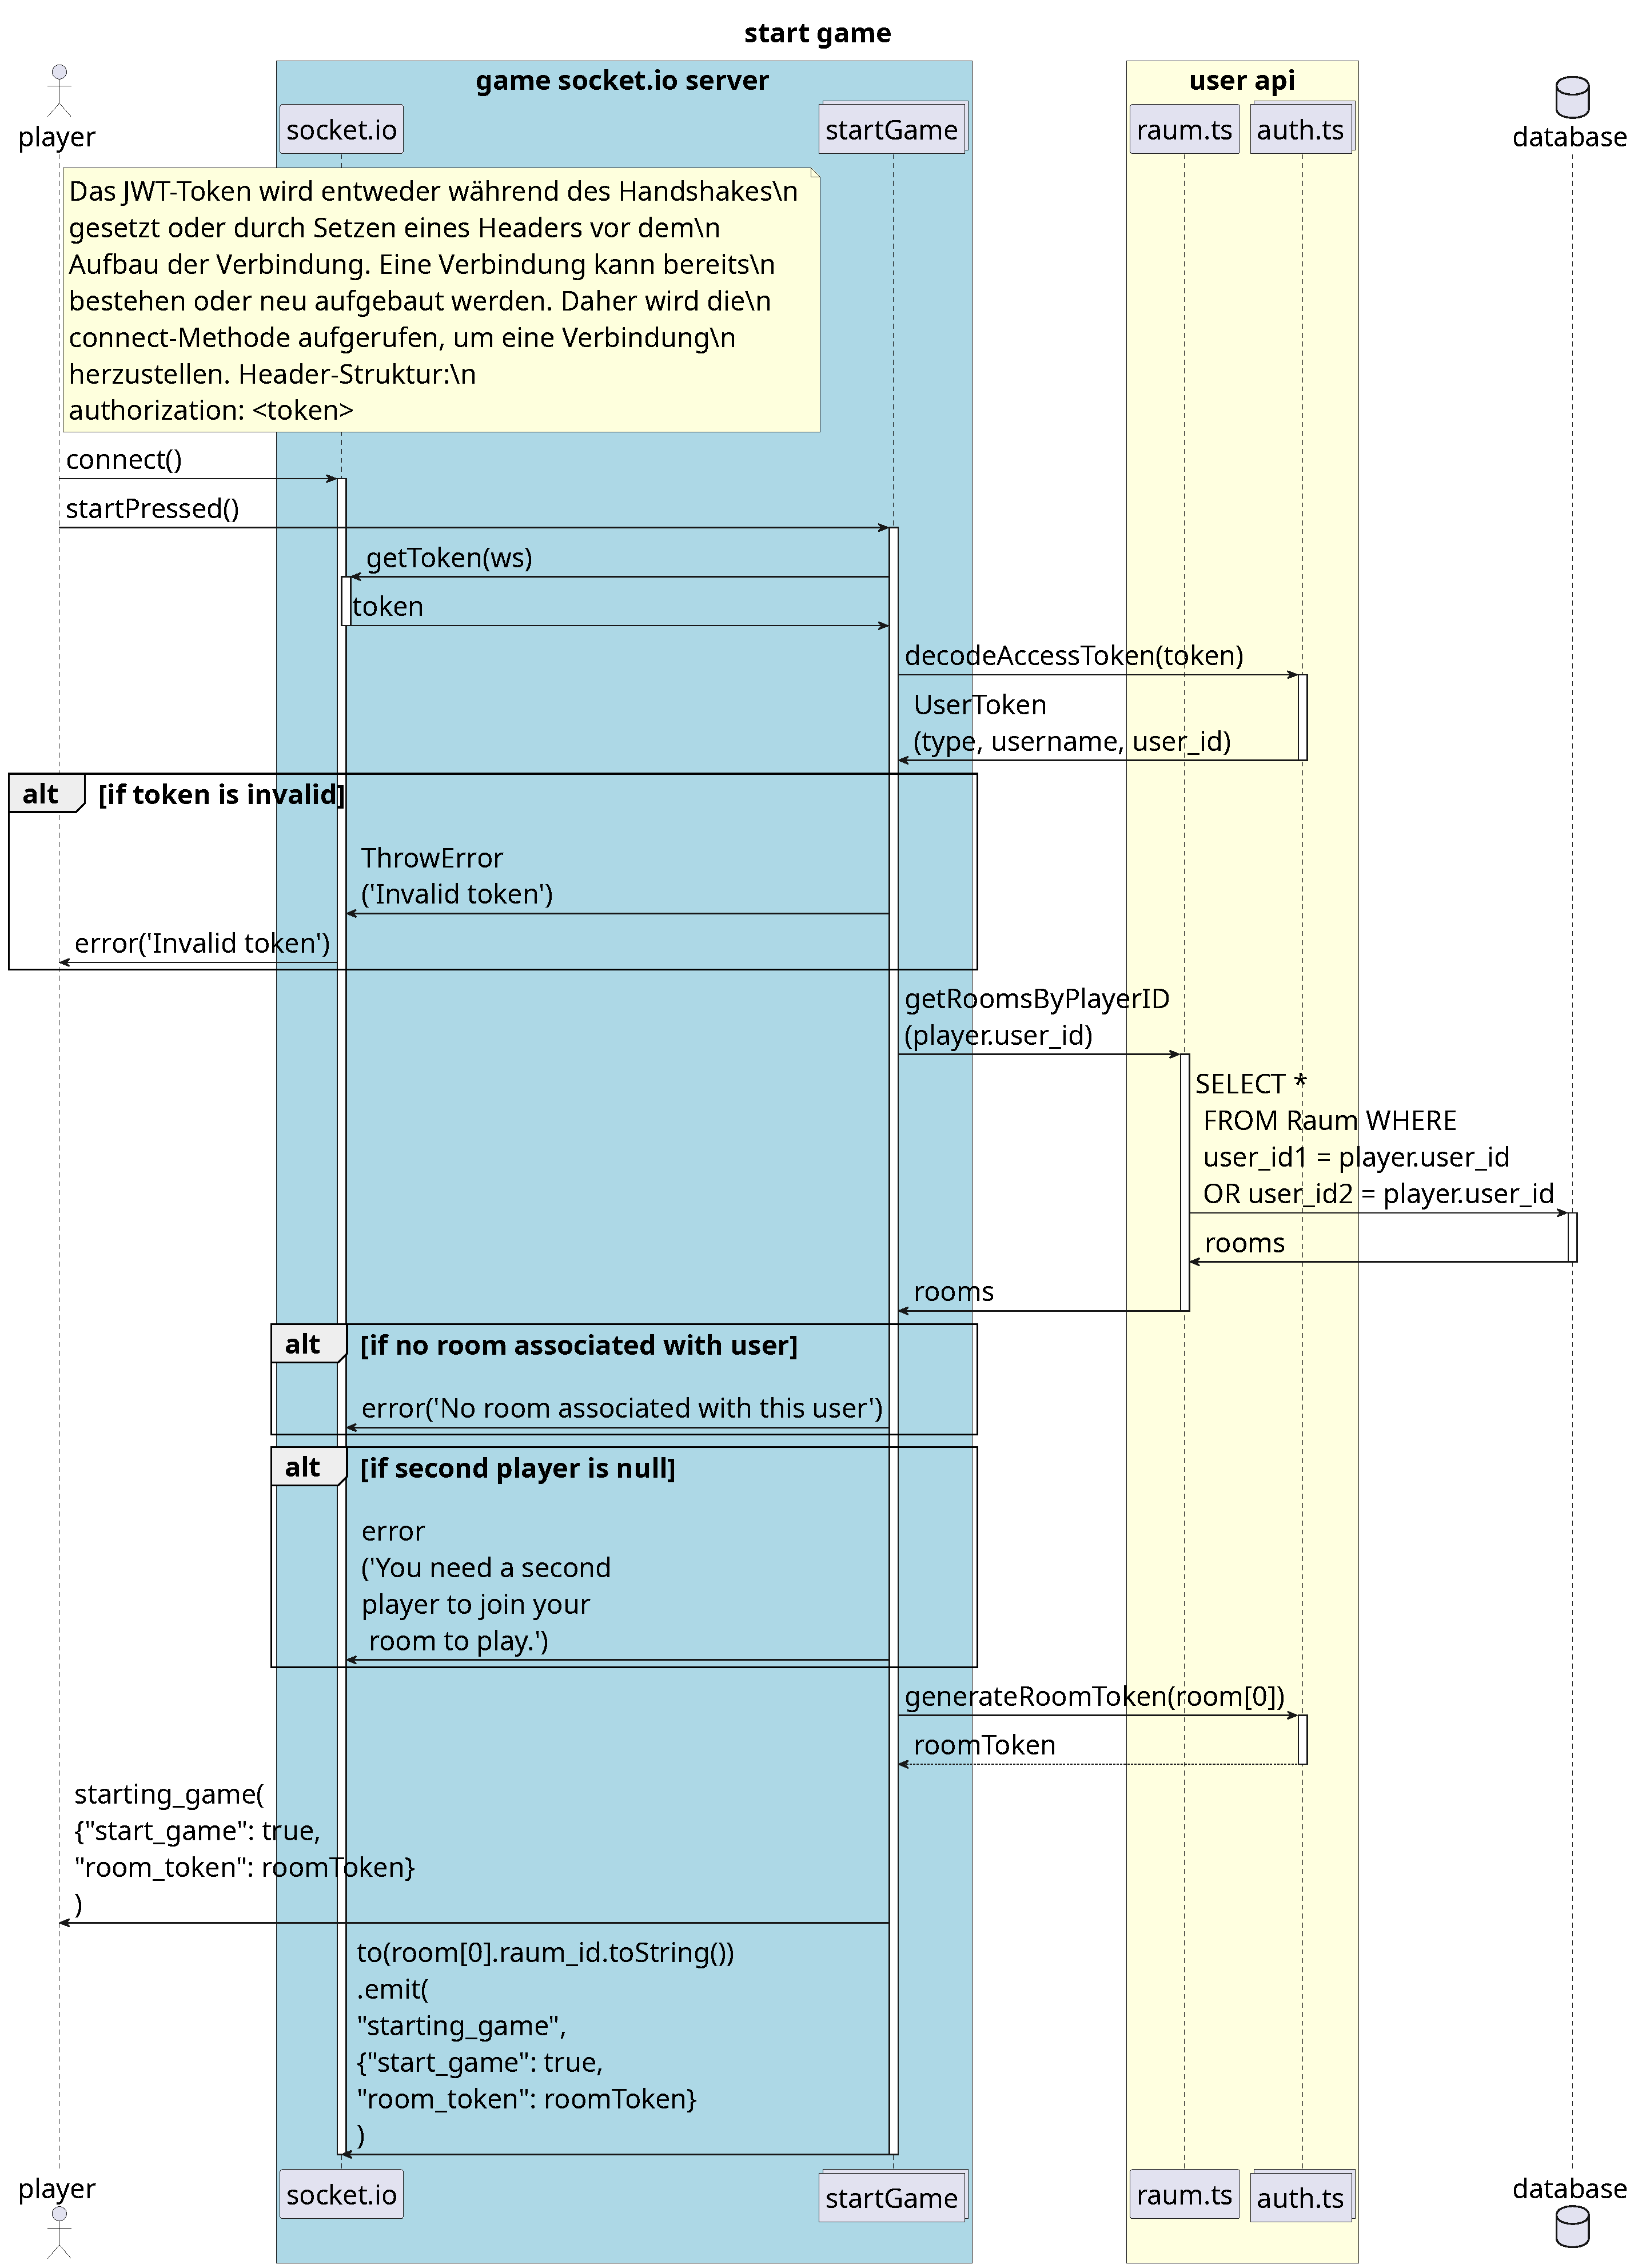
\includegraphics[width=\textwidth ]{resources/start_game.pdf}
	\caption{Dein TExt hier}
	\label{fig:ablaufdiagramm-start_game}
\end{figure}

\begin{figure}[H]
	\centering
	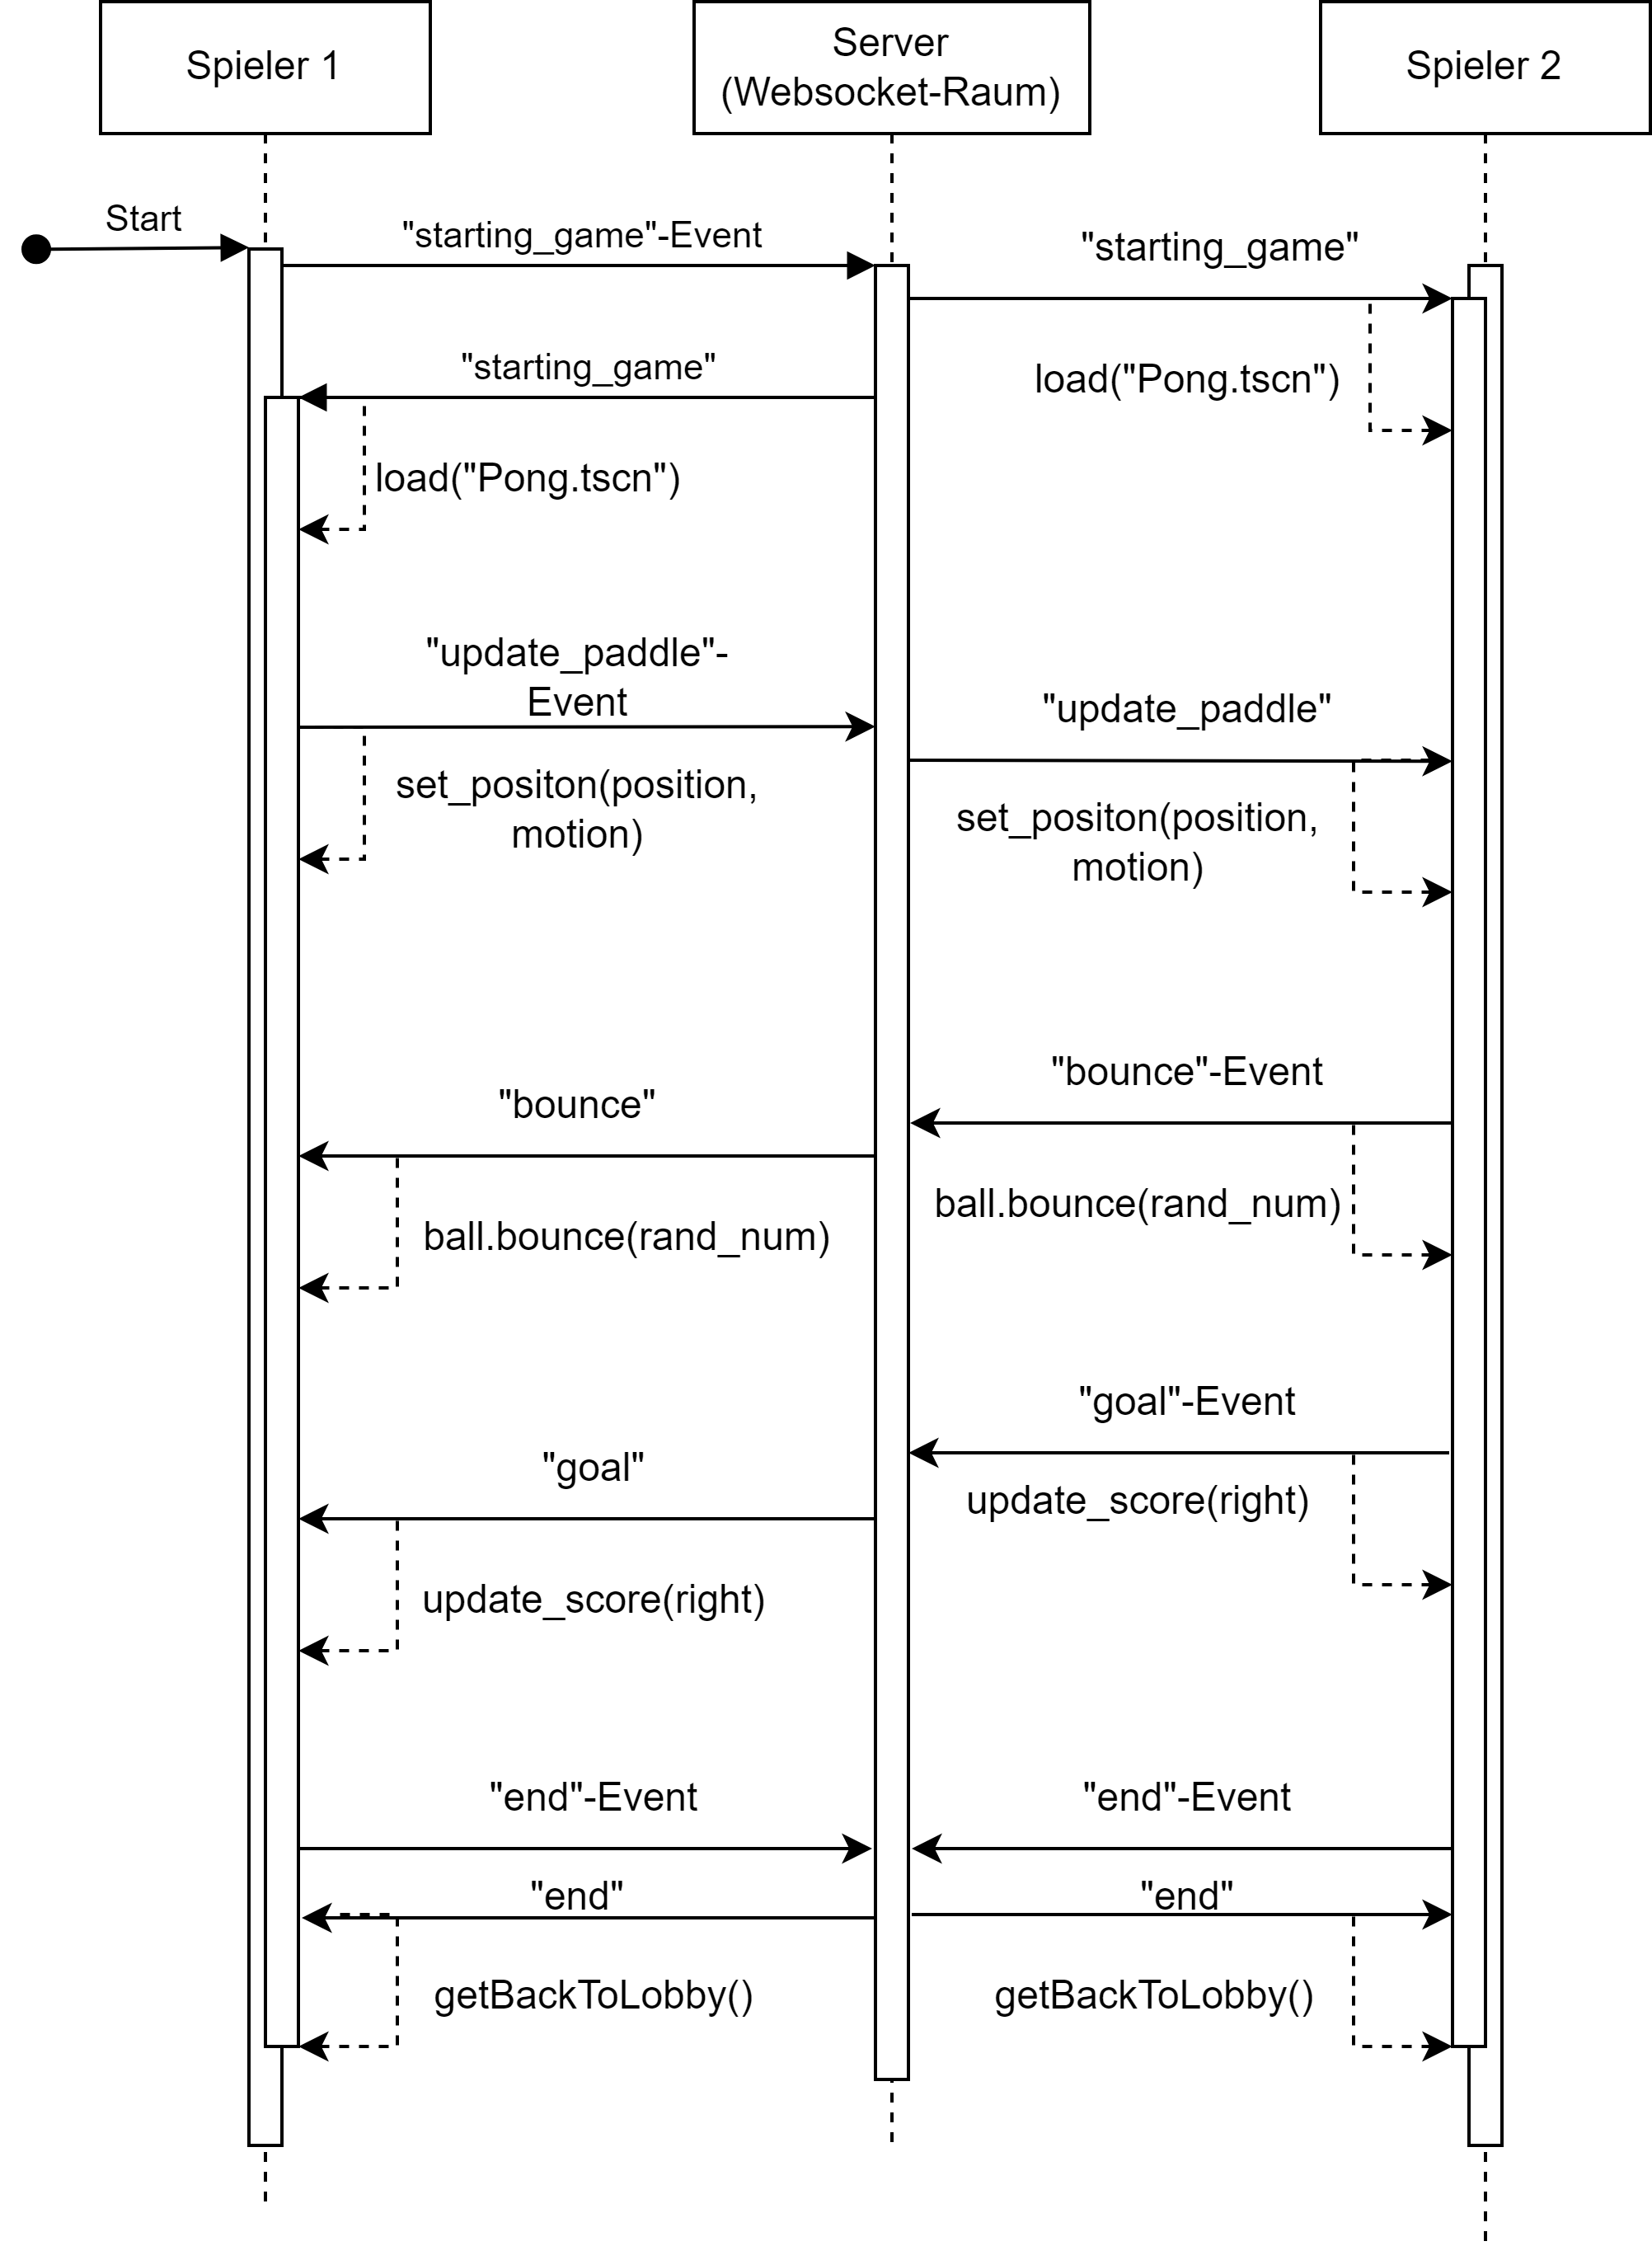
\includegraphics[width=\textwidth ]{resources/Event-Based-Spielablauf.png}
	\caption{Eventbasierter Ablauf des Spiels über einen Socket-IO Websocket. Es handelt sich um eine Vereinfachte Ansicht. Beide Seiten können die jeweiligen Events an den Server senden.}
	\label{fig:ablaufdiagramm-spiel}
\end{figure}

\subsection{Mögliche Alternativen}
Anstelle einer zentralisierten Architektur wäre ein dezentralisierter Ansatz möglich. Es könnte ein Peer-To-Peer System Implementiert werden. Anstelle von einem zentralen System ist jeder Client miteinander direkt verbunden \cite{gordon2001distributed}.

\section{Reflexion}

\subsection{Rückblick}
\begin{itemize}
    \item \textbf{Änderungen nach dem Projekt}: Was würde man im Nachhinein anders machen, um das System zu verbessern?
\end{itemize}

\subsection{Herausforderungen}
\begin{itemize}
    \item \textbf{Größte Herausforderungen}: Rückblick auf die bedeutendsten Schwierigkeiten und wie sie gelöst wurden.
\end{itemize}
\newpage
 \printbibliography[title={Quellen}]
\end{document}
